\documentclass[aspectratio=169]{beamer}\usepackage[utf8]{inputenc}
\usepackage[english]{babel}
\usepackage{color}
\usepackage{amsmath,mathtools}
\usepackage{mathptmx}
\usepackage[11pt]{moresize}
\setbeamertemplate{navigation symbols}{}
\setbeamersize{text margin left=5mm,text margin right=5mm}
\usepackage{wrapfig}
\usepackage{bbm}
\usepackage{xcolor}
\usepackage{tabularx}
\usepackage{bm}


\newcommand{\R}{\mathbb{R}}
\newcommand{\E}{\mathbb{E}}
\newcommand{\N}{\mathbb{N}}
\newcommand{\Z}{\mathbb{Z}}
\newcommand{\V}{\mathbb{V}}
\newcommand{\Q}{\mathbb{Q}}
\newcommand{\K}{\mathbb{K}}
\newcommand{\C}{\mathbb{C}}
\newcommand{\T}{\mathbb{T}}
\newcommand{\I}{\mathbb{I}}

\setbeamertemplate{caption}[numbered]

\title{Prediction of Power Generation}
\subtitle{ Waleed Alhaddad}

\begin{document}
\setbeamercolor{background canvas}{bg=blue!3}
\begin{frame}
\titlepage
\end{frame}
%
%\begin{frame}\frametitle{Model}
%
%\begin{equation}
%\begin{split}
%dX(t) &= a(X(t); \theta) dt + b (X(t); \theta ) dW(t) \quad t > 0 \\
%X(0) & = x_0
%\end{split}\label{main}
%\end{equation}
%where $X(t) \in [0,1]$ is the normalized stochastic analogue of the power generated $p(t)$. 
%
%\begin{enumerate}
%\item Drift is given by $a(X(t),t ; \theta) = - \theta (t) \Big(X(t)-p(t)\Big)$
%\item Non-centered diffusion is given by: $ b (X(t); \theta) = \sqrt{2\alpha(t) \theta (t) p(t) \Big(1-p(t)\Big) X(t) \Big(1-X(t)\Big)}  $
%\end{enumerate}
%
%\end{frame}


\begin{frame}[label=guide]\frametitle{ Reader's Guide }

List of changes in this iteration:
\begin{itemize}
\item Matched data with every forecast
\item Normalized according to installed power of each period
\item Interpolated the forecast using cubic splines.

\end{itemize}

Next steps:
\begin{itemize}
\item upgrade the numerical integrator and use the interpolated forecast
\item Check performace using the interpolated forecasts and data
\end{itemize}

Note :
\begin{itemize}
\item Green slides: possible future extensions
\item Red slides: notes to be removed
\end{itemize}

\end{frame}


\begin{frame}\frametitle{ Toy model with Synthetic Data }
We generate paths from an SDE  with given parameters using Monte Carlo simulation and then fit the model to check the retrievability of the parameters. We consider the following cases:
\begin{itemize}
\item[1:]  Constant parameter Wiener process: finite and infinite horizon.
\item[2:]  Controlled Wiener process within an interval.
\item[3:]  Controlled Wiener process centered around a given function. 
\end{itemize}
\end{frame}


\begin{frame}\frametitle{ Stochastic Differential Equation }
Given the SDE
\begin{equation}
\begin{split}
dX_t &= a(X_t; \bm{\theta}) dt + b (X_t; \bm{\theta} ) dW_t \quad t > 0 \\
X_0 & = x_0
\end{split}\label{main}
\end{equation}
Consider a set of N observations, $ X=\{ X_{t_0^N} , X_{t_1^N} ,\ldots , X_{t_N^N} \}$ observed within intervals $\Delta_N$. 

\begin{itemize}
\item $\Delta_N$: is any function of the number of samples, $N$. For example, $\Delta_N = \frac{1}{N}$.
\item $a(X_t; \bm{\theta})$ is the drift function \textcolor{brown}{(add technical conditions here)}
\item $b (X_t; \bm{\theta} )$ is the diffusion function \textcolor{brown}{(add technical conditions here)}
\item $\bm{\theta}$ is a vector of constant parameters
\end{itemize}
\end{frame}

\begin{frame}\frametitle{ likelihood function }
We have the Likelihood function of the transition density

\begin{equation}
\mathcal{L}(\theta;X) = \prod\limits_{i=1}^n\rho( {X_{i+1}|X_{i}}, \bm{\theta})  \rho(X_0) 
\end{equation}
Consider a Gaussian transition density,
\begin{equation*}
\mathcal{L}(\bm{\theta}; X) = \prod\limits_{i=1}^n  \frac{1}{\sqrt{2 \pi b(X_i,\bm{\theta})^2 dt}  } \exp\Big(\frac{-((X_{i+1}-X_i) - a(X_i,\bm{\theta}) dt )^2}{2b(X_i,\bm{\theta})^2 dt}\Big) \rho(X_0)
\end{equation*}

We take the improper prior $\rho(X_0)=1$.
\end{frame}

\begin{frame}\frametitle{ Case 1: Constant Parameters }
For a fixed $b(X_t; \bm{\theta})=\sigma$ and a fixed $a(X_t; \bm{\theta})=\mu$. We observe that varying the sampling and discretization parameters affects the convergence behavior.


We consider the following three situations:
\begin{enumerate}
\item[1.1] Infinite Horizon expansion caused by increasing samples N\\ ( increasing $N$ and $\Delta_N$ is fixed).
\item[1.2] Infinite Horizon expansion caused by increasing intervals $\Delta_N$ \\ ( fixed $N$ and increasing decreasing $\Delta_N$).
\item[1.3] Finite Horizon expansion with sample compression, i.e where $\Delta_N=\frac{T}{N}$ \\ (increasing $N$, fixed $T$).
\end{enumerate}
\end{frame}


\begin{frame}\frametitle{ Case 1: Implementation }

In the following, we use  L-BFGS-B algorithm to optimize the likelihood with bounds on $\sigma$ being positive. And we use $\mu=100$ and $\sigma=10$ for the path generation. We denote the estimators of $\mu$ and $\sigma$ by  $\hat{\mu}$ and $\hat{\sigma}$ where,

\begin{equation}
 \hat{\mu} = \arg \underset{\mu \in \R}{\max} \ \mathcal{L}(\bm{\theta};X) \quad \quad  \quad \quad \hat{\sigma} = \arg \underset{\sigma \in \R^+}{\max} \mathcal{L}(\bm{\theta};X)
\end{equation}

\end{frame}


\begin{frame}%\frametitle{ Case 1: Scenario illustration }
The above cases can be seen clearly in the illustration below.
\begin{figure}
  \includegraphics[scale=0.4]{Figures/data_horizons.pdf}
  %\label{fig:boat1}
\end{figure}
\end{frame}





%\begin{itemize}
%\item $ \sigma (X(t); \theta) = \sqrt{2 p(t) \Big(1-p(t)\Big) X(t) \Big(1-X(t)\Big)}  $
%\item $b(X(t),t ; \theta) = -  \Big(X(t)-p(t)\Big)$
%\end{itemize}

\begin{frame}\frametitle{ Case 1.1: Constant Parameters \\
 Infinite Horizon expansion caused by increasing samples N }
An increase of the number of samples $N$ in a growing time interval $T$. In this case, we obtain  convergence of the order $\frac{1}{\sqrt{N}}$ as expected.

\begin{figure}
  \includegraphics[scale=0.45]{Figures/case11v2.pdf}
  \caption{convergence in the case of infinite horizon expansion caused by increasing samples N}
  %\label{fig:boat1}
\end{figure}

\end{frame}

\begin{frame}\frametitle{ Case 1.2: Constant Parameters \\
 Infinite Horizon expansion caused by increasing intervals dt }
In this case, the estimator $\hat{\sigma}$ of the diffusion coefficient is inconsistent. This is because the time interval between the samples is increasing and so we do not have as much information about the variation of the process. However, the drift estimator $\hat{\mu}$ is still consistent. We have not seen any theoretical proof of this situation.

\begin{figure}
  \includegraphics[scale=0.45]{Figures/case12v3.pdf}
  \caption{convergence rate in the case of infinite horizon expansion caused by increasing intervals $\Delta_N$}
  %\label{fig:boat1}
\end{figure}

\end{frame}


\begin{frame}\frametitle{ Case 1.3: Constant Parameters \\
 Finite Horizon expansion with sample compression }
In this case, we observe increasing number of  samples in a fixed time interval (sample compression).In this case the drift estimator $\mu$ is inconsistent while the diffusion estimator $\sigma$ is consistent. This situation  matches the theoretical discussion in [1].

\begin{figure}
  \includegraphics[scale=0.45]{Figures/case13v2.pdf}
  \caption{Convergence rate in the case of finite horizon expansion with sample compression  }
  %\label{fig:boat1}
\end{figure}

We will see next that there are no consistent estimators of the drift  term $b(X(t), \theta)$ in this case. 

\end{frame}


\begin{frame}\frametitle{ Remarks }
\begin{enumerate}
\item  It is easier to obtain convergence in the diffusion coefficient. Because the estimator of the diffusion has access to  information from the infinite variation of the wiener process while the drift does not. We can show this theoretically from the efficiency condition of the estimators.
\item The convergence generally follows Monte Carlo's convergence rate in terms of sampling as expected. This statement is wrong in a high frequency setting, as we have different convergence rate for estimator of the diffusion and than for the estimator of the drift as we will see next. The estimator of the drift converges slower than the Monte Carlo rate given that both are consistent.
\end{enumerate}

\end{frame}

\begin{frame}\frametitle{Motivation of high frequency SDE data}

High frequency situations are not uncommon and extreme  but may happen for data that looks reasonable. For instance, in some cases  weekly data is treated as high frequency data . A situation is considered high frequency with respect to the amount of  variation in the drift term [1] (or in regards to the speed at which it reverts to the mean).  \\

This also important for building confidence intervals as the limiting distribution of our estimator may not be Gaussian. For example, in the setting of high frequency data and fixed time $T$ (case 1.3 above) the limiting distribution of the estimator is path dependent and is given by a normal variance-mixture distribution which can be heavy tailed with no finite moments [1]. However, in this case, a  modification of the estimator can help in achieving  a Gaussian limiting distribution of the estimator.

Please note that in the setting of high frequency SDE data, we have two possibilities:
\begin{itemize}
\item Finite Horizon (fixed time $T$): this corresponds to case 1.3 above.
\item Infinite Horizon: this corresponds to other two cases.
\end{itemize}


\end{frame}

\begin{frame}\frametitle{Convergence of the drift estimator for high frequency  SDE  \\(Case 1.3 / Finite Horizon)}

In a high frequency setting with finite horizon (case 1.3), there are \textbf{no} consistent estimators of the drift term $a(X_t, \bm{\theta})$ (see [1]) as we break the following condition :\\

Given the following SDE,
\begin{equation}
\begin{split}
dX_t &= a(X_t; \alpha) dt + b(X_t; \beta ) dW_t \quad t > 0 \\
X(0) & = x_0
\end{split}\label{main}
\end{equation}

the drift estimator  $\hat{\alpha}$ of the parameter set $\alpha$ of the system is consistent if and only if
\begin{equation}
n \Delta_n \to \infty  \label{conv_cond}
\end{equation}
And this condition contradicts having a finite horizon as we trivially have $T=N \Delta_N \to \infty$. If the  condition (\ref{conv_cond}) is not satisfied, we cannot have a consistent estimator  $\hat{\alpha}$ of the drift. However, the estimator $\hat{\beta}$ of the diffusion term $b (X_t; \beta)$ is still consistent regardless. 
\end{frame}



\begin{frame}\frametitle{Convergence of the drift estimator for high frequency  SDE  \\(Case 1.3 / Finite Horizon)}
To show this result numerically, we pick any $\Delta_n$ such that $T=n \Delta_n \to \infty$. In this example, we modify the non-consistent  drift parameter estimator (case $1.3$) such that 
\begin{equation}
dt=\frac{T}{N} \quad  \rightarrow  \quad dt=\frac{T}{\sqrt{N}}
\end{equation}
Then we recover back the convergence of the other cases as this replacement turns the finite horizon to an infinite horizon. 
\end{frame}


\begin{frame}\frametitle{Numerical Convergence for high frequency  SDE}
In this numerical example, we take $\Delta_N = \frac{T}{\sqrt{N}}$ as an example.
\begin{equation}
\text{Finite Horizon:} \ dt=\frac{T}{N} \quad  \text{versus} \quad \text{Infinite Horizon:} \ dt=\frac{T}{\sqrt{N}}
\end{equation}
We confirm  condition (\ref{conv_cond}) numerically. It is clear that in the finite horizon case the estimator of the diffusion $\hat{\sigma}$ converges while the estimator of the drift $\hat{\mu}$ is not consistent. Whereas, in the infinite horizon case, we obtain the expected convergence in both parameters.
\begin{figure}
  \includegraphics[scale=0.35]{Figures/case13v2.pdf}
   \includegraphics[scale=0.35]{Figures/case13infinite.pdf}
  \caption{Right side: Finite horizon with $dt=\frac{T}{N}$, Left side: Infinite horizon with $dt=\frac{T}{\sqrt{N}}$   }
  %\label{fig:boat1}
\end{figure}

\end{frame}





\begin{frame}\frametitle{Convergence for high frequency SDE data}
We can show that the score function of the likelihood is an efficient martingale estimating function and that the obtained estimator is optimal\footnote{If we consider an approximate martingale estimator function such as the pseudo likelihood, then we require an extra condition that $n \Delta_n^{2 \kappa - 1} \to 0 $ where $\kappa$ is the order of $\Delta_N$ in RHS of the expectation (\ref{expec_martin})}. Then we have the following convergence rates [3]:

For a finite Horizon (fixed T)
\begin{equation}
\hat{\alpha} \text{ is not consistent } \quad \text{and} \quad relative \ error(\hat{\beta}) \propto \frac{1}{\sqrt{N}}
\end{equation}
For an infinite Horizon ($T \to \infty$)
\begin{equation}
relative \ error(\hat{\alpha})  \propto \frac{1}{\sqrt{N\Delta_N}} \quad \text{and} \quad  relative \ error(\hat{\beta}) \propto \frac{1}{\sqrt{N}} 
\end{equation}
Note that the estimator $\hat{\alpha}$ of the drift is affected by the time discretization while the estimator $\hat{\beta}$ of the diffusion is independent of the time discretization.

\end{frame}


\begin{frame}\frametitle{High Frequency  SDE General Convergence }
Consider a set of N observations, $X= \{ X_{t_0^N} , X_{t_1^N} ,\ldots , X_{t_N^N} \}$ and the following martingale estimator function,
\begin{equation}
G_n(\gamma) = \sum\limits_{i=1}^N g(\Delta_N , X_{t_{i}^N},X_{t_{i-1}^N} ; \gamma )
\end{equation}
where $t_{i}^n = i \Delta_n $, $\gamma = (\alpha, \beta)$ and $g=(g_1, g_2)$ .
In our martingale case\footnote{The results can also be adapted to a non martingale estimating function such as a pseudo likelihood},we must have,
\begin{equation}
E_\gamma \Big(    g(\Delta_N , X_{t_{i}^N},X_{t_{i-1}^N} ; \gamma) \Big| X_{t_{i-1}^N}  \Big) = 0
\label{expec_martin}
\end{equation} where the $\hat{\beta}$ estimator is given by solving $ G_n(\gamma) = 0 $.

\end{frame}

{
\setbeamercolor{background canvas}{bg=green!30}

\begin{frame}\frametitle{High Frequency  SDE -  Possible Extensions}

\begin{itemize}
\item Try to understand the limit of when we need to switch to the high frequency from the low frequency regime. That is how it depends on the speed of the  mean reversion in our model.
\item Get the martingale estimator function of the Gaussian transition density explicitly.
\item State the optimality and efficiency of the estimators explicitly.
\item Obtain the stated theoretical convergence rate.
\item Try to show theoretically why in case 1.2 , the diffusion estimator is not consistent.
\item Understand and state the conditions under which we have a unique parameter estimation to our SDE.
\end{itemize}

\end{frame}
}


\begin{frame}\frametitle{References}
\begin{itemize}
\item[][1] Jakobsen, N. M., \& Sørensen, M. (2017). Efficient estimation for diffusions sampled at high frequency over a fixed time interval. Bernoulli, 23(3), 1874-1910. doi:10.3150/15-bej799
\item[][2] Sørensen, M. (2007). Efficient Estimation for Ergodic Diffusions Sampled at High Frequency. SSRN Electronic Journal. doi:10.2139/ssrn.1150694
\item[][3] Kessler, M., Lindner, A., \& Sørensen, M. (2012). Statistical methods for stochastic differential equations. Boca Raton, FL: Chapman \& Hall/CRC.
\end{itemize}

\end{frame}


\begin{frame}\frametitle{ Paths as IID samples  }

We have the Likelihood function of the transition density

\begin{equation}
\mathcal{L}(\theta;X) = \prod\limits_{j=1}^M\prod\limits_{i=1}^N\rho( {X_{j,i+1}|X_{j,i}}, \bm{\theta})  \rho(X_0) 
\end{equation}
Consider a Gaussian transition density,
\begin{equation*}
\mathcal{L}(\bm{\theta}; X) = \prod\limits_{j=1}^M \prod\limits_{i=1}^N  \frac{1}{\sqrt{2 \pi b(X_{j,i};\bm{\theta})^2 dt}  } \exp\Big(\frac{-((X_{j,i+1}-X_{j,i}) - a(X_{j,i};\bm{\theta}) dt )^2}{2b(X_{j,i};\bm{\theta})^2 dt}\Big) \rho(X_0)
\end{equation*}

We take the improper prior $\rho(X_0)=1$.

\end{frame}

\begin{frame}\frametitle{ Paths as IID samples - Implementation }

As before, we use  L-BFGS-B algorithm to optimize the likelihood with bounds on $\sigma$ being positive. We denote the estimators of $\mu$ and $\sigma$ by  $\hat{\mu}$ and $\hat{\sigma}$ where,

\begin{equation}
 \hat{\mu} = \arg \underset{\mu \in \R}{\max} \ \mathcal{L}(\bm{\theta};X) \quad \quad  \quad \quad \hat{\sigma} = \arg \underset{\sigma \in \R^+}{\max} \mathcal{L}(\bm{\theta};X)
\end{equation}

\end{frame}

\begin{frame}\frametitle{ Paths as IID samples - Convergence }
We have Monte Carlo convergence in terms of samples as expected.
\begin{figure}
  \includegraphics[scale=0.5]{Figures/conv_M_unbounded.pdf}
   \includegraphics[scale=0.5]{Figures/conv_N_unbounded.pdf}
  \caption{ Optimized using L-BFGS-B algorithm. True parameters used are $\mu = 100$ and $\sigma = 10$.M is the number of paths and N is the number of samples.    }
  %\label{fig:boat1}
\end{figure}

\end{frame}



\begin{frame}\frametitle{Case 2: Controlled Wiener process in a unit box }
We have the SDE,
\begin{equation}
\begin{split}
dX_t &= a(X_t; \bm{\theta}) dt + b (X_t; \bm{\theta} ) dW_t \quad t > 0 \\
X_0 & = 0
\end{split}\label{main}
\end{equation}
Consider a set of N observations, $X= \{ X_{t_0^N} , X_{t_1^N} ,\ldots , X_{t_N^N} \}$ on intervals of $\Delta_N$.\\ We choose,
\begin{equation}
a_{i+1}(X_i; \bm{\theta})= \mu X_i(\frac{1}{2} - X_i)  \quad \quad b_{i+1} (X_i; \bm{\theta} )=\sigma X_i (1-X_i)
\end{equation}
We choose $ 0<\sigma <<1$ and $\mu\in (0,1]$. Then, we have contained the Wiener process in the interval $[0,1]$ with high probability.

\end{frame}


\begin{frame}\frametitle{Case 2: Controlled Wiener process in a unit box }
We see that the process is contained within the unit box as we kill the diffusion coefficient if we touch the boundary. Additionally, the drift coefficient is always directed towards the center line $\frac{1}{2}$ of the unit box.
\begin{figure}
  \includegraphics[scale=0.45]{Figures/Wiener_box.pdf}
  \caption{ With  high probability the wiener process stays inside the box as $\mu \in (0,1]$ and $\sigma << 1$ }.
  %\label{fig:boat1}
\end{figure}

\end{frame}


\begin{frame}\frametitle{Case 2: Controlled Wiener process in a unit box - Parameter Inference }

We obtain the same convergence as before,

\begin{figure}
  \includegraphics[scale=0.5]{Figures/conv_M_box.pdf}
   \includegraphics[scale=0.5]{Figures/conv_N_box.pdf}
  \caption{Optimized using L-BFGS-B algorithm. True parameters used are $\mu = 0.5$ and $\sigma = 0.1$. M is the number of paths and N is the number of samples.   }
  %\label{fig:boat1}
\end{figure}

\end{frame}


\begin{frame}\frametitle{Case 3: Controlled Wiener process around a given function }
We have the SDE,
\begin{equation}
\begin{split}
dX_t &= a(X_t; \bm{\theta}) dt + b (X_t; \bm{\theta} ) dW_t \quad t > 0 \\
X_0 & = 0
\end{split}\label{main}
\end{equation}
Consider a set of N observations, $X= \{ X_{t_0^N} , X_{t_1^N} ,\ldots , X_{t_N^N} \}$ on intervals of $\Delta_N$.\\ We choose,
\begin{equation}
a_{i+1}(X_i; \bm{\theta})= \mu X_i(\frac{1}{2}(1 + p_i )- X_i)  \quad \quad b_{i+1} (X_i; \bm{\theta} )=\sigma X_i (1-X_i)
\end{equation}
We choose $ 0<\sigma <<1$ and $\mu\in (0,1]$. Then, we have contained the Wiener process in the interval $[0,1]$ with high probability. Additionally, we add mean reversion to $\frac{1}{2}(1 + p_i ) $ where  $p_i = \sin(\frac{i}{N} 2\pi)$.


\end{frame}

\begin{frame}\frametitle{Case 3: Controlled Wiener process following a given function }
We see that the process follows the sine wave  closely when the  drift parameter $\mu \approx 1$ and that we have a shift artifact when the drift parameter $\mu<<1$. Note that the process does not  escape the unit box as the diffusion is controlled and the drift is directed towards the function which is always inside the unit box.
\begin{figure}
  \includegraphics[scale=0.4]{Figures/Wiener_sine_box.pdf}
   \includegraphics[scale=0.4]{Figures/conv_sine_shift.pdf}
  \caption{Illustrative examples: On the right, we see the controlled wiener process responding to the boundary  by killing the diffusion at the peaks of the sine wave. On the right we observe an unintended  shift artifact when the drift parameter $\mu<<1$.   }
  %\label{fig:boat1}
\end{figure}

\end{frame}

\begin{frame}\frametitle{Case 3: Controlled Wiener process around a function - Paramter Inference }
We obtain the same convergence as before,

\begin{figure}
  \includegraphics[scale=0.5]{Figures/conv_M_sine.pdf}
   \includegraphics[scale=0.5]{Figures/conv_N_sine.pdf}
  \caption{ Optimized using L-BFGS-B algorithm. True parameters used are $\mu = 100$ and $\sigma = 10$.M is the number of paths and N is the number of samples.    }
  \label{fig:sine}
\end{figure}

\end{frame}



\begin{frame}\frametitle{ Case 4: Following deterministic functions }
As we construct processes that follow or revert to deterministic function it is natural to state the SDE in terms of deviations from the deterministic function. Then, we have for $V_t= X_t - p_t$

\begin{equation}
\begin{split}
dV_t &= a(V_t; \bm{\theta}_t) dt + b (V_t; \bm{\theta}_t ) dW_t \quad t > 0 \\
V_0 & = v_0
\end{split}\label{main_V}
\end{equation}

where we choose $ a(V_t; \bm{\theta}_t) = - \theta_t V_t$ to have mean reversion with exponential speed in time controlled by some strictly positive parameter $\theta_t$. To keep the process within a unit box, we choose $ b (V_t; \bm{\theta} )= \sqrt{ 2 \alpha_t \theta_t p_t (1-p_t)X_t (1-X_t)   }$

\end{frame}


\begin{frame}\frametitle{ Case 4: Implementation }
In the previous sections we relied on the Euler discretization of SDEs in order to obtain our estimators through the Maximum Likelihood approach. However, this introduces errors in the likelihood similar to the observed error in the wiener process following the sine wave in (\ref{fig:sine}). To prevent such artifacts, we solve for the moments of the process defined by the SDE in (\ref{main_V}). We have,

\begin{equation}
\begin{split}
\E [V_t^k] &=  \E \Big[ \Big( \int a(V_t; \bm{\theta}_t) dt + \int b (V_t; \bm{\theta}_t ) dW_t \Big)^k \Big] \quad t > 0 \\
V_0 & = v_0
\end{split}\label{main_V_expectations}
\end{equation}
For a Gaussian approximation, we are interested in the first two moments.

\end{frame}


\begin{frame}\frametitle{ Case 4: Implementation - first moment }
The first moment $(k=1)$ is given by,

\begin{equation}
\begin{split}
 m_1(t) =\E V_t &=  \E \Big[  \int a(V_t; \bm{\theta}_t) dt \Big] + \E \Big[ \int b (V_t; \bm{\theta}_t ) dW_t  \Big] \\
 & = \E \Big[  \int a(V_t; \bm{\theta}_t) dt \Big]
\end{split}\label{main_V_1_moment}
\end{equation}
In our case, the drift is linear and is given by $ a(V_t; \bm{\theta}_t) = - \theta_t V_t$. then, we have 
\begin{equation}
\begin{split}
 & m_1(t) =\E V_t =     \Big[  \int - \theta_t \E V_t dt \Big] 
 \iff \frac{dm_1(t)}{dt}=    - \theta_t m_1(t) \ \ ; \quad m_1(0)=\E[V_0]= v_0
\end{split}\label{main_V_1_moment}
\end{equation}
This is an ODE which has solutions of the form, 
\begin{equation}
m_1(t) = v_0 \exp ( - \int_0^t \theta_s \ ds ) 
\end{equation}

\end{frame}

\begin{frame}\frametitle{ Case 4: Implementation - second moment }
The second moment $(k=2)$ is given by,

\begin{equation}
\begin{split}
  =\E V_t^2 &=  \E \Big[ \Big( \int a(V_t; \bm{\theta}_t) dt + \int b (V_t; \bm{\theta}_t ) dW_t \Big)^2 \Big] \\
\end{split}\label{main_V_2_moment}
\end{equation}
Let $Y_t=g(V_t)=V_t^2$ then $g_t= 0 , \ g^{'} (V_t) = 2V_t$ and $g^{''} (V_t) = 2$. Using $It\hat{o}$ and Taylor, 
\begin{equation}
\begin{split}
dY_t =  \frac{\partial g}{\partial t} dt &+  \frac{\partial g}{\partial v} \Big(a (V_t; \bm{\theta}_t ) \ dt + b (V_t; \bm{\theta}_t ) dW_t  \Big)\\
& + \frac{1}{2} \frac{\partial^2 g}{\partial v^2} \Big(a (V_t; \bm{\theta}_t ) \ dt + b (V_t; \bm{\theta}_t ) dW_t  \Big)^2 + \mathcal{O}(dV_t^3)
\end{split}
\end{equation}
As $dt \to 0$, we have
\begin{equation}
\begin{split}
dY_t &=  \frac{\partial g}{\partial t} + \Big( a (V_t; \bm{\theta}_t ) \frac{\partial g}{\partial v}  + \frac{b^2 (V_t; \bm{\theta}_t )}{2} \frac{\partial^2 g}{\partial v^2} \Big) dt + b (V_t; \bm{\theta}_t ) \frac{\partial g}{\partial v} dW_t  \\
&= 2\Big( a (V_t; \bm{\theta}_t ) V_t  + \frac{b^2 (V_t; \bm{\theta}_t )}{2}  \Big) dt +  2V_t b (V_t; \bm{\theta}_t ) dW_t
\end{split}
\end{equation}

\end{frame}



\begin{frame}\frametitle{ Case 4: Implementation - second moment }
The second moment $(k=2)$ is given by,

\begin{equation}
\begin{split}
\E [V_t^2] =  \E Y_t &= 2  \E\Big[ \int \Big( a (V_t; \bm{\theta}_t ) V_t  + \frac{b^2 (V_t; \bm{\theta}_t )}{2}  \Big) dt \Big] +  2 \E \Big[ \int V_t b (V_t; \bm{\theta}_t ) dW_t \Big]\\
&= 2  \E\Big[ \int \Big( a (V_t; \bm{\theta}_t ) V_t  + \frac{b^2 (V_t; \bm{\theta}_t )}{2}  \Big) dt \Big]\\
\end{split}
\end{equation}
In our case, the drift is $ a(V_t; \bm{\theta}_t) = - \theta_t V_t$ and the diffusion is given by $ b (V_t; \bm{\theta} )= \sqrt{ 2 \alpha_t \theta_t p_t (1-p_t)X_t (1-X_t)   } =  \sqrt{ 2 \alpha_t \theta_t p_t (1-p_t)(V_t + p_t) (1-V_t-p_t)   }$. Then,
\begin{equation*}
\begin{split}
m_{2}&(t)=\E [V_t^2] = 2  \int \Big( - \theta_t \E[V_t^2]  +  \alpha_t \theta_t p_t (1-p_t)\E[(V_t + p_t) (1-V_t-p_t) ] \Big) dt \\
&=2  \int \Big( - \theta_t \E[V_t^2]  +  \alpha_t \theta_t p_t (1-p_t)( p_t(1 - p_t) +(1-2p_t)\E[V_t] - \E[V_t^2] ) \Big) dt \\
&=2  \int \Big( -\E[V_t^2] [\theta_t + \alpha_t \theta_t p_t(1-p_t) ] + \E[V_t][\alpha_t \theta_t p_t (1-p_t) (1-2p_t)] + \alpha_t \theta_t p_t^2(1-p_t)^2 \Big) dt \\
\end{split}
\end{equation*}

\end{frame}


\begin{frame}\frametitle{ Case 4: Implementation - second moment }
The second moment $m_2(t)$ is given by solving the ODE,

\begin{equation*}
\begin{split}
\frac{d m_{2}(t)}{dt}&=2 \Big( -m_{2}(t) [\theta_t + \alpha_t \theta_t p_t(1-p_t) ] + m_{1}(t)[\alpha_t \theta_t p_t (1-p_t) (1-2p_t)] + \alpha_t \theta_t p_t^2(1-p_t)^2 \Big) \\
\end{split}
\end{equation*}
where $m_2(0) = \E[V_0^2] = v_0^2$ and has a solution of the form,
\begin{equation*}
\begin{split}
&m_{2}(t) = m_{2}(0) \exp \Big( -2 \int_0^t  [\theta_\tau + \alpha_\tau \theta_\tau p_\tau(1-p_\tau) ] \ d\tau  \Big) + \\
& 2 \int\limits_{0}^{t}   \exp \Big( -2 \int_0^s  [\theta_\tau + \alpha_\tau \theta_\tau p_\tau(1-p_\tau) ] \ d\tau \Big) \Big( m_{1}(t-s)[\alpha_{t-s} \theta_{t-s} p_{t-s} (1-p_{t-s}) (1-2p_{t-s})]  \\
& + \alpha_{t-s} \theta_{t-s} p_{t-s}^2(1-p_{t-s})^2 \Big)  \  ds
\end{split}
\end{equation*}

\end{frame}



\begin{frame}\frametitle{Following deterministic functions - Cases }

We consider the following cases:
\begin{itemize}
\item[4.1] Constant parameters $\bm{\theta}_t = \bm{\theta} $
	\begin{itemize}
	\item[4.1.1] reverting to a constant function
	\item[4.1.2] reverting to a deterministic function
	\end{itemize}
\item[4.2] Time dependent parameters $\bm{\theta}_t$
\end{itemize}

\end{frame}






\begin{frame}\frametitle{ Case 4.1: Following deterministic functions - constant parameters }
In this case, the first moment  $m_1(t)$ reduces to, 

\begin{equation}
m_1(t) = v_0 \exp ( -t\theta ) 
\end{equation}
And the second moment $m_2(t)$ reduces to,

\begin{equation*}
\begin{split}
&m_{2}(t) = m_{2}(0) \exp \Big( -2  [t \theta + \alpha \theta \int_0^t    p_\tau (1-p_\tau)  \ d\tau ] \Big) + \\
& 2 \int\limits_{0}^{t}    \exp \Big( -2 [s \theta + \alpha \theta \int_0^s    p_\tau (1-p_\tau)  \ d\tau ] \Big) \Big( m_{1}(t-s)[\alpha \theta p_{t-s} (1-p_{t-s}) (1-2p_{t-s})]  \\
& + \alpha \theta p_{t-s}^2(1-p_{t-s})^2  \Big) \  ds
\end{split}
\end{equation*}


\end{frame}


\begin{frame}\frametitle{ Case 4.1.1: Following a constant function - constant parameters }
For constant forecast $p_t = \frac{1}{2}$ the second moment reduce further, 

\begin{equation*}
\begin{split}
&m_{2}(t) = m_{2}(0) \exp \Big( -2 t \theta (1 + \frac{\alpha }{4} ) \Big) +   \frac{\alpha \theta}{8} \int\limits_{0}^{t}  \exp \Big( -2 s \theta (1 + \frac{\alpha }{4} )\Big) \  ds \\
& =m_{2}(0) \exp \Big( -2 t \theta (1 + \frac{\alpha }{4} ) \Big) + \frac{\alpha }{16 (1+ \frac{\alpha}{4})} \Big(1- \exp ( -2 t \theta (1 + \frac{\alpha }{4} ) \Big) 
\end{split}
\end{equation*}
Then the variance is given by,
\begin{equation}
\V[V_t] =m_{2}(0) \exp \Big( -2 t \theta (1 + \frac{\alpha }{4} ) \Big) + \frac{\alpha }{16 (1+ \frac{\alpha}{4})} \Big(1- \exp ( -2 t \theta (1 + \frac{\alpha }{4} ) \Big)   - v_0^2 \exp ( -2t\theta ) 
\end{equation}
Note that the second moment $m_2(0)=v_0^2$ as the previous point $V_{t_{i-1}}=v_0$ deterministic.
%% CHANGE ALL zero lower bounds to t_{i-1} 
\end{frame}


\begin{frame}\frametitle{ Case 4.1.1: Following a constant function - constant parameters }

To conclude, we have the following mean and variance functions,

\begin{equation}
\begin{split}
\E[V_{t_i}| V_{t_{i-1}}=v_0] &= v_0 \exp ( -(t_i - t_{i-1})\theta ) \\
 \V[V_{t_i}| V_{t_{i-1}}=v_0] &= \frac{\alpha }{16 (1+ \frac{\alpha}{4})} \Big(1- \exp ( -2 (t_i - t_{i-1}) \theta (1 + \frac{\alpha }{4} ) \Big) \\
\end{split}
\end{equation}

Next, we discretize  and obtain the likelihood.
\end{frame}


\begin{frame}\frametitle{ Case 4.1.1: Following a constant function - constant parameters }
To obtain the likelihood, consider a set of N observations, $X= \{ X_{t_0^N} , X_{t_1^N} ,\ldots , X_{t_N^N} \}$ on intervals of $\Delta_N$. We have $V=X-\frac{1}{2}$ .  Then,

\begin{equation}
\begin{split}
\E[V_{i}| V_{i-1}=v_0] &= v_0 \exp ( -\Delta_N \theta )  \\
 \V[V_{i}| V_{i-1}=v_0] &= \frac{\alpha }{16 (1+ \frac{\alpha}{4})} \Big(1- \exp ( -2 \Delta_N\theta (1 + \frac{\alpha }{4} ) \Big)\\
\end{split}
\end{equation}

The Likelihood  of the transition density is given by,

\begin{equation}
\mathcal{L}(\theta;X) = \prod\limits_{j=1}^M\prod\limits_{i=1}^N\rho( {V_{j,i+1}|V_{j,i}}, \bm{\theta}) 
\end{equation}
And the Gaussian transition density,
\begin{equation*}
\mathcal{L}(\bm{\theta}; V) = \prod\limits_{j=1}^M \prod\limits_{i=1}^N  \frac{1}{\sqrt{2 \pi \V[V_{j,t_i}| V_{j,t_{i-1}}=v_0] }  } \exp\Big(\frac{-(V_{j,i+1}   - \E[V_{j,t_i}| V_{j,t_{i-1}}=v_0] )^2}{2\V[V_{t_i}| V_{j,t_{i-1}}=v_0]}\Big) 
\end{equation*}

\end{frame}


\begin{frame}\frametitle{ Case 4.1.1: Following a constant function - constant parameters }
We obtain the following convergence using the analytical moments obtained from the $V_t$ process and enforcing that the parameters $\theta$ and $\alpha$ are non-negative.

\begin{figure}
   \includegraphics[scale=0.22]{Figures/conv_M_moments_constant_func_sym.jpg}
    \includegraphics[scale=0.22]{Figures/conv_N_moments_constant_fun_symjpg.jpg}
  \caption{This is done for true parameters $\theta = 0.5$ and $\alpha=1$ using  L-BFGS-B optimization algorithm }
  %\label{fig:boat1}
\end{figure}
\end{frame}


\begin{frame}\frametitle{ Case 4.1.1: Following a constant function - constant parameters }
Further, we note that the  inference on the drift needs special care in situations of high speed reversion to the mean. Such situations seem to occur in the following cases:
\begin{itemize}
\item  $ \theta > > 1$  and big enough $\alpha$
\item  $\Delta_N > > 1$ 

\end{itemize}
In both cases, we see a flattening in the likelihood in the direction of the drift parameter $\theta$ which  causes the optimizer to return inconsistent estimates of the drift parameter $\theta$. These two cases are applicable if the function or the process oscillates at a high frequency with respect to the other.

\end{frame}


\begin{frame}\frametitle{ Case 4.1.1: Following a constant function - constant parameters }

\begin{figure}
    \includegraphics[scale=0.22]{Figures/sample_moments_constant_func_1_01.pdf}
    \includegraphics[scale=0.22]{Figures/sample_moments_constant_func_10_01.pdf}
      \includegraphics[scale=0.22]{Figures/sample_moments_constant_func_100_01.pdf}
      
    \includegraphics[scale=0.22]{Figures/conv_M_moments_constant_func_1_01.pdf}
    \includegraphics[scale=0.22]{Figures/conv_M_moments_constant_func_10_01.pdf}
      \includegraphics[scale=0.22]{Figures/conv_M_moments_constant_func_100_01.pdf}
      
          \includegraphics[scale=0.22]{Figures/conv_N_moments_constant_fun_1_01.pdf}
    \includegraphics[scale=0.22]{Figures/conv_N_moments_constant_fun_10_01.pdf}
      \includegraphics[scale=0.22]{Figures/conv_N_moments_constant_fun_100_01.pdf}
      
  \caption{We can see how an increase of $\theta >>1$ with big enough $\alpha$ causes sharp oscillations that make the inference of  $\theta$ unfeasible.  }
  %\label{fig:boat1}
\end{figure}
\end{frame}


\begin{frame}\frametitle{ Case 4.1.1: Following a constant function - constant parameters }
In the second case of increasing $\Delta_N$, we see the following flattening of the likelihood in the direction of $\theta$.
\begin{figure}
    \includegraphics[scale=0.5]{Figures/dt_increasing_moments.pdf}
      
  \caption{We can see how an increase of time intervals $\Delta_N >>1$  causes a flattening of the likelihood making the valley of the optimal $\theta$ shallower  until the  inference of  $\theta$ becomes unfeasible.  }
  %\label{fig:boat1}
\end{figure}
\end{frame}


\begin{frame}\frametitle{ Case 4.1.1: Following a constant function - constant parameters }

Question: How can we quantify the mean reversion of an SDE   ?  \\

The reversion to the mean is not only determined by the parameter $\theta$ but also by the diffusion term. We can see this in the following example,

\begin{equation}
dX_t = (1+X_t)dt + (1+X_t^2) dW_t
\end{equation}

which at first glance does not seem mean reverting, but in fact,  it is mean reverting. The reversion is driven  solely  by diffusion term in this case.  This is a case of volatility induced stationary, as the non-linearity in the diffusion term are responsible for the mean reversion. A similar non-linearity is present in our model and quantifying the effective mean reversion  will help determine if we are in the convergent regime  where our estimator of the drift is consistent or not.

Regarding, the specific application to wind forecasts this should not be an issue as the forecast and the recorded data are unlikely to oscillate around each other at a "high" frequency.


\end{frame}

\begin{frame}\frametitle{ Case 4.1.1: Following a constant function - constant parameters }

Answer: Yes, it is true that such SDE's are stationary even though they are not "mean reverting". The  "mean reversion" or the "pull" is induced solely by the diffusion term. We can show that 

\begin{equation}
dX_t = (1+X_t)dt + (1+X_t^2) dW_t
\end{equation} 
is stationary. Even though its associated process with constant diffusion $\sigma$
\begin{equation}
dX_t = (1+X_t)dt + \sigma dW_t
\end{equation}
is clearly non-stationary. We can do that using the tools we will introduce next to check and find the stationary distributions of our SDEs. Namely, using the scale and speed densities. 
\end{frame}




\begin{frame}\frametitle{ Case 5.1.1: Theoretical Background }
Consider an SDE,
\begin{equation}
\begin{split}
dX_t &= a(X_t; \bm{\theta}) dt + b (X_t; \bm{\theta} ) dW_t \quad t > 0 \\
X_0 & = x_0
\end{split}\label{main}
\end{equation}
We define the scale density $s(x)$,
\begin{equation}
s(x) = exp \Big[ \int^x - \frac{2  a(y; \bm{\theta})}{b^2 (y; \bm{\theta} )}\ dy \Big]
\end{equation}
And the speed density $m(x)$,
\begin{equation}
m(x) = \frac{1}{b^2 (y; \bm{\theta}) \  s(x)}
\end{equation}
 
\end{frame}

\begin{frame}\frametitle{ Case 5.1.1: Theoretical Background }


A unique stationary distribution of the process $X_t$ exists if and only if 
\begin{equation}
\int_{x_0}^r s(x) \ dx = \infty \quad \int_{l}^{x_0} s(x) \ dx = \infty \quad \int_l^r m(x) \ dx < \infty
\end{equation}
where $x_0 \in (l,r)$ and $(l,r)$ is an interval where $b^2 (y; \bm{\theta} ) > 0$

\end{frame}


\begin{frame}\frametitle{ Case 5.1.1: Theoretical Background }
Considering the  SDE of a process following a constant forecast $p$,
\begin{equation}
\begin{split}
dX_t &= -\theta(X_t - p) dt + \sqrt{2 \theta \alpha p(1-p) X_t (1-X_t)} dW_t \quad t > 0 \\
X_0 & = x_0
\end{split}\label{main}
\end{equation}
We obtain the scale density $s(x)$ with integrability condition $\frac{p}{a} \leq -1 $ and $\frac{1-p}{a} \leq -1$
\begin{equation}
s(x) = exp \Big[ \int^x - \frac{2  a(y; \bm{\theta})}{b^2 (y; \bm{\theta} )}\ dy \Big] = exp \Big[ \int^x_{x_0}  \frac{y-p}{a y (y-1)}\ dy \Big]  \propto (1-x)^{\frac{1-p}{a}} x^{p/a}
\end{equation}
where $a= - \alpha p(1-p) <0$.Then the speed density $m(x)$ becomes, 
\begin{equation}
m(x) = \frac{1}{b^2 (y; \bm{\theta}) \  s(x)} \propto (1-x)^{-\frac{1-p}{a}-1} x^{-\frac{p}{a}-1}
\end{equation}
We note that $(l,r) = (-\infty, \infty)$ is where $b^2 (y; \bm{\theta} ) >0$. Let $x_0 \in (l,r)$. Taking $x_0=1$ we see that
\begin{equation}
\int_{x_0}^r s(x) \ dx = \infty \quad \int_{l}^{x_0} s(x) \ dx = \infty \quad \int_l^r m(x) \ dx < \infty
\end{equation}
\end{frame}

\begin{frame}\frametitle{ Case 5.1.1: Theoretical Background }
Under the condition,
\begin{equation}
\begin{cases}
\frac{p}{a} \leq -1\\
\frac{1-p}{a} \leq -1\\
\end{cases}\iff
\min (p, 1-p) \geq -a \iff  \min (p, 1-p) \geq \alpha p(1-p)
\end{equation}
For example, if forecast is constant $ p = \frac{1}{2}$, the condition becomes $\alpha \leq 2$.

we conclude that there exists a unique stationary distribution of  $X_t$ and its proportional to the speed density,
\begin{equation}
m(x)\propto (1-x)^{-\frac{1-p}{a}-1} x^{-\frac{p}{a}-1}
\end{equation}
 which is the kernal of a Beta distribution with shape parameters
\begin{equation}
  Beta \ \Big( \frac{p}{\alpha (1-p)}, \frac{1}{\alpha p } \Big)
\end{equation}
\end{frame}


\begin{frame}\frametitle{ Case 5.1.1: Theoretical Background }
Now we consider the centered process $V_t= X_t - p$,
\begin{equation}
\begin{split}
dX_t &= -\theta V_t dt + \sqrt{2 \theta \alpha p(1-p) (V_t +p ) (1-V_t-p)} dW_t \quad t > 0 \\
X_0 & = x_0
\end{split}\label{main}
\end{equation}
We obtain the scale density $s(x)$,
\begin{equation}
s(x) = exp \Big[ \int^x - \frac{2  a(y; \bm{\theta})}{b^2 (y; \bm{\theta} )}\ dy \Big] = exp \Big[ \int^x_{x_0} \frac{y-p}{a y^2 + by +c}\ dy \Big]  
\end{equation}
where,
\begin{equation}
\begin{cases}
a&=  \alpha p(1-p)\\
b&=  \alpha p(1-p)(2p-1)\\
c&=  \alpha p^2(1-p)^2\\
\end{cases}
\end{equation}
\end{frame}



\begin{frame}\frametitle{ Case 5.1.1: Theoretical Background }
To simplfy, we choose the constant forecast to be $p=\frac{1}{2}$. Then we have,

\begin{equation}
\begin{cases}
a&=  \frac{\alpha}{4} \\
b&=  0 \\
c&=  \frac{\alpha}{16} \\
\end{cases}
\end{equation}
and the scale density becomes, 
\begin{equation}
\begin{split}
s(x) &= exp \Big[ \int^x - \frac{2  a(y; \bm{\theta})}{b^2 (y; \bm{\theta} )}\ dy \Big] = exp \Big[ \int^x_{x_0} \frac{y}{a y^2 +c}\ dy \Big] =exp \Big[ \int^x_{x_0} \frac{y}{\frac{\alpha }{16}+\frac{\alpha  y^2}{4}}\ dy \Big]\\
& \propto \left(4 v^2+1\right)^{2/\alpha } \quad \quad (\alpha >0)
\end{split}
\end{equation}
Then we have the speed density $m(x)$,
\begin{equation}
m(x) = \frac{1}{b^2 (y; \bm{\theta}) \  s(x)} \propto \left(4 v^2+1\right)^{-\frac{\alpha +2}{\alpha }}
\end{equation}
\end{frame}


\begin{frame}\frametitle{ Case 5.1.1: Theoretical Background }
We proceed to check if it is stationary. 

We note that $(l,r) = (-\infty, \infty)$ is where $b^2 (y; \bm{\theta} ) >0$. Let $x_0 \in (l,r)$. Taking $x_0=0$, we see that
\begin{equation}
\int_{x_0}^r s(x) \ dx = \infty \quad \int_{l}^{x_0} s(x) \ dx = \infty \quad \int_l^r m(x) \ dx < \infty
\end{equation}
So we conclude that it is a stationary distribution of $V_t$ and its unique.
Hence, the kernal of the invarient distribution of the process $V_t$ with constant forecast $p=\frac{1}{2}$ is $\pi(v)= \frac{\sqrt{\pi} \  \Gamma (\frac{1}{2}+ \frac{2}{\alpha})}{\Gamma(\frac{2+\alpha}{\alpha})}\left(1+4 v^2\right)^{-\frac{\alpha +2}{\alpha }}$. Note that it almost resembles a t-student distribution.
\end{frame}



\begin{frame}\frametitle{ Case 5.1.1: Theoretical Background }


\begin{figure}
    \includegraphics[scale=0.9]{Figures/invarient_Vt.pdf}
  \caption{ The stationary distribution $\pi(v)$ of the process $V_t$ is symmetric with heavy tails.}
  %\label{fig:boat1}
\end{figure}

\end{frame}



\begin{frame}\frametitle{Following deterministic functions - Cases }

In an improved model, we incorperate  Beta density transitions. We repeat the same cases as follows:
\begin{itemize}
\item[5.1] Constant parameters $\bm{\theta}_t = \bm{\theta} $
	\begin{itemize}
	\item[5.1.1] reverting to a constant function
	\item[5.1.2] reverting to a deterministic function
	\end{itemize}
\item[5.2] Time dependent parameters $\bm{\theta}_t$
\end{itemize}

However, first lets discuss why and how do we incorperate the Beta transition densities.

\end{frame}


\begin{frame}\frametitle{ Case 5.1.1: Following a constant function - constant parameters }
Recall that both $X_t$ and $V_t$ are controlled processes that are constrained within a unit box. The symmetry of the Gaussian transition density of these two processes indicate that we have some probability outside the unit box once the forecast touches the boundry. There are many ways to fix this behaviour:
\begin{enumerate}
\item Use a Beta transition density for all the transitions while matching the moments of the Gaussian transition density.
\item Use a Beta transition density only when the transition density of the process touches the boundry of the unit box.This depends on the width and position of the transition density.
\begin{enumerate}
\item match the parameters of the Beta transition with the moments of the Gaussian transition.
\item Not to match the moments of the Gaussian and introdude the beta parameters as two additional hyperparameters (increasing the degrees of freedom).
\end{enumerate}
\end{enumerate}

\end{frame}

\begin{frame}\frametitle{ Case 5.1.1: Following a constant function - constant parameters }

If we like to enforce that the Beta transition matches the moments of the Gaussian, then
we can solve for the paramters of the Beta distribution in terms of the parameters of the Gaussian transition density.

First, lets consider the non-centered process $X_t$. In that case, we choose standard Beta distribution which has support on $x \in [0,1]$. Then solving for its parameters in terms of the parameters of the Gaussian transition denisty, to obtain

\begin{equation} 
\alpha = \Big(  \frac{1-\tilde{\mu}}{\tilde{\sigma}^2} -\frac{1}{\tilde{\mu}}   \Big)\tilde{\mu}^2 \quad \quad \beta =  \alpha \Big(\frac{1}{\tilde{\mu}} -1 \Big)
\end{equation}
where $\tilde{\sigma}^2$ is the variance of the Gaussian transition density of the process and $\tilde{\mu}$ is its mean.
\end{frame}

\begin{frame}\frametitle{ Case 5.1.1: Following a constant function - constant parameters }
To ensure the existence of such a Beta distribution with the parameters required
\begin{equation} 
\alpha = \Big(  \frac{1-\tilde{\mu}}{\tilde{\sigma}^2} -\frac{1}{\tilde{\mu}}   \Big)\tilde{\mu}^2 \quad \quad \beta =  \alpha \Big(\frac{1}{\tilde{\mu}} -1 \Big)
\end{equation}
we have the followind conditions by the definition of the standard Beta distribution:
\begin{enumerate}
\item $x \in [0,1]$.
\item Its shape parameters $\alpha$ and $\beta$ must be positive definite.
\end{enumerate}
Solution (this only applies to Euler realizations due to time discretization):
\begin{enumerate}
\item Discard realizations $X_t$ outside the range $(0,1)$.
\item Ensure that $\alpha >0$ and $\beta >0 $ with high probability.
\end{enumerate}
The first condition is automatically satisfied with high probability. The second condition introduces the following restrictions:
\begin{equation}
\alpha >0 ,\ \beta >0 \iff  0< \tilde{\mu}_t < 1  \ \text{and} \  \tilde{\sigma}_t^2 < \tilde{\mu}_t - \tilde{\mu}_t^2
\end{equation}
while the first restriction $ 0< \tilde{\mu}_t < 1$ holds with very high probability. The second restricts the second moment of the process $X_t$ not to exceed its mean,  i.e $\E[X_t^2] \leq \tilde{\mu}_t \quad \forall t$
\end{frame}

\begin{frame}\frametitle{ Case 5.1.1: Following a constant function - constant parameters }
Next, we consider the centered process $V_t$. Since the process $V_t$ is  inside the range $(-1,1)$ with high probability, the standard Beta distribution cannot model its transitions. Therefore, we translate the distribution to have support on $[a,b]=[-1,1]$.  We use the linear transformation $y= g(x)= a + (b-a) x $ then we have
\begin{equation}
\  g^{-1}(y)= \frac{a-y}{b-a} \quad \text{and} \quad \Big| \frac{\partial g^{-1}(y)}{\partial y }  \Big| = \frac{1}{b-a}
\end{equation}
And the general Beta distribution becomes, 
\begin{equation}
f_Y(y)= f_X(g^{-1}(y) ) \Big| \frac{\partial g^{-1}(y)}{\partial y }  \Big| = \frac{1}{B(\alpha, \beta) (b-a)} \Big(\frac{a-y}{b-a}\Big)^{\alpha -1}\Big(1-\frac{a-y}{b-a} \Big)^{\beta -1}
\end{equation}
and we have,
\begin{equation}
\E[Y]= a + (b-a) \E[X] = a + (b-a) \frac{\alpha}{\alpha + \beta}
\end{equation}
\begin{equation}
\V[Y]= (b-a)^2 \V[X] = (b-a)^2 \frac{\alpha \beta}{(\alpha + \beta)^2 (\alpha + \beta + 1)}
\end{equation}
\end{frame}

\begin{frame}\frametitle{ Case 5.1.1: Following a constant function - constant parameters }
Next, we need to solve the system in terms of the mean and variance of the process $V_t$.
\begin{equation}
\begin{cases}
\tilde{\mu}_t=a + (b-a) \frac{\alpha}{\alpha + \beta}\\
\tilde{\sigma}_t^2= (b-a)^2 \frac{\alpha \beta}{(\alpha + \beta)^2 (\alpha + \beta + 1)}\\
\end{cases}
\end{equation}
to obtain, 
\begin{equation}
\alpha = \frac{(\tilde{\mu}_t-a) \left(\tilde{\mu}_t^2-\tilde{\mu}_t (a+b)+\tilde{\sigma}_t^2+a b\right)}{\tilde{\sigma}_t^2 (a-b)}
\end{equation}

\begin{equation}
\beta = \frac{(\tilde{\mu}_t-b) \left(\tilde{\mu}_t^2-\tilde{\mu}_t (a+b)+\tilde{\sigma}_t^2+a b\right)}{\tilde{\sigma}_t^2 (b-a)}
\end{equation}
then for our interval of interest $[a,b]=[-1,1]$, we have

\begin{equation}
\alpha = - \frac{(1+\tilde{\mu}_t )(\tilde{\mu}_t^2 + \tilde{\sigma}_t^2 -1)}{2 \tilde{\sigma}_t^2} \quad \quad \beta =  \frac{(\tilde{\mu}_t-1 )(\tilde{\mu}_t^2 + \tilde{\sigma}_t^2 -1)}{2 \tilde{\sigma}_t^2} \label{param_transformed_beta}
\end{equation}

\end{frame}

\begin{frame}\frametitle{ Case 5.1.1: Following a constant function - constant parameters }
As before, for the general Beta distribution on the interval $[a,b]=[-1,1]$, we must have that
\begin{enumerate}
\item $x \in [-1,1]$.
\item Its shape parameters $\alpha$ and $\beta$ must be positive definite.
\end{enumerate}
Solution (this only applies to Euler realizations due to time discretization):
\begin{enumerate}
\item Discard realizations $V_t$ outside the range $(-1,1)$.
\item Ensure that $\alpha >0$ and $\beta >0 $ with high probability.
\end{enumerate}
The first condition is automatically satisfied with high probability. The second condition introduces the following restrictions:
\begin{equation}
\alpha >0 ,\ \beta >0 \iff  0< \tilde{\mu}_t < 1  \ \text{and} \  \tilde{\sigma}_t^2 < 1 - \tilde{\mu}_t^2
\end{equation}
while the first restriction $ -1< \tilde{\mu}_t < 1$ holds with very high probability. The second restricts the second moment of the process $V_t$ not to exceed one,  i.e.  $\E[V_t^2] \leq 1 \quad \forall t$
\end{frame}


\begin{frame}\frametitle{ Case 5.1.1: Following a constant function - constant parameters }
If we approximate all transitions by a Beta transition density, we obtain the log-likelihood, 
\begin{equation}
\ell(\bm{\theta}; V)= \sum\limits_{j=1}^M \sum\limits_{i=1}^N (\alpha -1)\log(V_{j,i+1}) + (\beta -1) \log(1-V_{j,i+1}) - \log (B(\alpha, \beta))
\end{equation}
where $B(\alpha, \beta)=\frac{\Gamma (\alpha)\Gamma (\beta)}{\Gamma (\alpha + \beta)}$ is the Beta function. And enforcing to match the transition moments of the Gaussian, we have
\begin{equation} 
\alpha = \Big(  \frac{1-E[V_{j,t_i}| V_{j,t_{i-1}}=v_0]}{\V[V_{t_i}| V_{j,t_{i-1}}=v_0]} -\frac{1}{E[V_{j,t_i}| V_{j,t_{i-1}}=v_0]}   \Big)E[V_{j,t_i}| V_{j,t_{i-1}}=v_0]^2 \label{alph}
\end{equation}

\begin{equation} 
 \beta =  \alpha \Big(\frac{1}{\E[V_{j,t_i}| V_{j,t_{i-1}}=v_0]} -1 \Big) \label{gam}
\end{equation}
\end{frame}


\begin{frame}\frametitle{ Case 5.1.1: Following a constant function - constant parameters }
Another approach is to only approximate by a Beta distribution if the transition density of $X_t$ is sufficiently crossing the boarder of the unit box. For example, we approximate by a Beta the samples that satisfy either of the following conditions,
\begin{equation}
\begin{cases}
\mu_{t_i} + 3 \sigma_{t_i} >1\\
\mu_{t_i} - 3 \sigma_{t_i} <0
\end{cases} \iff
\begin{cases}
E[V_{j,t_i}| V_{j,t_{i-1}}=v_0] + p + 3 \sqrt{\V[V_{t_i}| V_{j,t_{i-1}}=v_0]} >1\\
E[V_{j,t_i}| V_{j,t_{i-1}}=v_0]+p - 3 \sqrt{\V[V_{t_i}| V_{j,t_{i-1}}=v_0]} <0
\end{cases}
\end{equation}

If a sample $V_{j,t_{i-1}}$ satisfies either of these conditions, we denote it by $\bar{V}_{j,t_{i-1}}$ and the number of such samples by $\bar{N}$.



%where $B(\alpha, \beta)=\frac{\Gamma (\alpha)\Gamma (\beta)}{\Gamma (\alpha + \beta)}$ is the Beta function.
%\begin{equation} 
%\alpha = \Big(  \frac{1-E[V_{j,t_i}| V_{j,t_{i-1}}=v_0]}{\V[V_{t_i}| V_{j,t_{i-1}}=v_0]} -\frac{1}{E[V_{j,t_i}| V_{j,t_{i-1}}=v_0]}   \Big)E[V_{j,t_i}| V_{j,t_{i-1}}=v_0]^2 
%\end{equation}
%
%\begin{equation} 
% \beta =  \alpha \Big(\frac{1}{\E[V_{j,t_i}| V_{j,t_{i-1}}=v_0]} -1 \Big)
%\end{equation}
\end{frame}

\begin{frame}\frametitle{ Case 5.1.1: Following a constant function - constant parameters }
We then construct the following likelihood,


\begin{equation}
\mathcal{L}(\theta;X) = \prod\limits_{j=1}^M \left[ \prod\limits_{i=1}^{N-\bar{N}}\rho( {V_{j,i+1}|V_{j,i}}, \bm{\theta}) \prod\limits_{i=1}^{\bar{N}} \bar{\rho}( {\bar{V}_{j,i+1}|\bar{V}_{j,i}}, \bm{\theta}) \right]
\end{equation}

and the log-likelihood becomes, 
\begin{equation}
\begin{split}
\ell(\bm{\theta}; V)&= \sum\limits_{j=1}^M \Big(  \sum\limits_{i=1}^{\bar{N}} (\alpha -1)\log(\bar{V}_{j,i+1}) + (\beta -1) \log(1-\bar{V}_{j,i+1}) - \log (B(\alpha, \beta))\\
&+ \sum\limits_{i=1}^{N-\bar{N}} - \frac{(V_{j,i+1}   - \E[V_{j,t_i}| V_{j,t_{i-1}}=v_0] )^2}{2\V[V_{t_i}| V_{j,t_{i-1}}=v_0]} - \frac{1}{2} \Big(2 \pi \V[V_{j,t_i}| V_{j,t_{i-1}}=v_0] \Big) \Big)
\end{split}
\end{equation}
where $\alpha$ and $\beta$ are given as in (\ref{alph}) and (\ref{gam}).

\end{frame}


\begin{frame}\frametitle{ Case 5.2.1: Time dependent Forecast  }
We approximate all transitions by a Beta transition density, we obtain the log-likelihood, 
\begin{equation}
\ell(\bm{\theta}; V)= \sum\limits_{j=1}^M \sum\limits_{i=1}^N (\alpha -1)\log(\frac{V_{j,i+1}+1}{2}) + (\beta -1) \log(1-\frac{V_{j,i+1}+1}{2}) - \log ( 2 B(\alpha, \beta))
\end{equation}

where $\alpha$ and $\beta$ are given as in (\ref{param_transformed_beta}):

\begin{equation}
\alpha = - \frac{(1+\tilde{\mu}_t )(\tilde{\mu}_t^2 + \tilde{\sigma}_t^2 -1)}{2 \tilde{\sigma}_t^2} \quad \quad \beta =  \frac{(\tilde{\mu}_t-1 )(\tilde{\mu}_t^2 + \tilde{\sigma}_t^2 -1)}{2 \tilde{\sigma}_t^2} \label{param_transformed_beta}
\end{equation}
where we compute the moments numerically before each realization using Euler
\begin{equation}
\tilde{\mu} = V_{j,i-1}e^{- \Delta N \theta}
\end{equation}
\begin{equation}
\begin{split}
\tilde{\sigma}_t^2 =  V_{j,i-1}^2 +& 2\Delta N (-V_{j,i-1}^2(\theta+\alpha\theta p_i (1-p_i) )  + \\
& V_{j,i-1}(\alpha\theta p_i(1-p_i)(1-2p_i )) + \alpha\theta p_i^2(1-p_i)^2) - \tilde{\mu}^2
\end{split}
\end{equation}
where $p_i$ is the discretization of the time dependent forecast.

\end{frame}


\begin{frame}\frametitle{ Case 5.2.1: Time dependent Forecast  }
We generate samples using the previous Euler scheme to numerically compute the moments before each realization.We obtain the following sample paths
\begin{figure}
    \includegraphics[scale=0.33]{Figures/sample_paths_beta_flex_0503.pdf}
        \includegraphics[scale=0.33]{Figures/sample_paths_beta_flex_0505.pdf}
      
  \caption{ Sample Paths using Beta transitions LHS: $\theta = 0.5$ and time dependent path variablitiy $\alpha (t) =  \alpha p_t (1-p_t)$ where $\alpha=0.3$. RHS:  $\theta = 0.5$, $\alpha=0.5$   }
  %\label{fig:boat1}
\end{figure}

\end{frame}

\begin{frame}\frametitle{ Case 5.2.1: Time dependent Forecast  }
We perform a convergence test for speed of reversion parameter $\theta = 0.5$ and time dependent path variablitiy $\alpha (t) =  \alpha p_t (1-p_t)$ where $\alpha=0.3$. We obtain the following convergence result
\begin{figure}
    \includegraphics[scale=0.4]{Figures/conv_M_beta_flex_10.pdf}
    \includegraphics[scale=0.4]{Figures/conv_N_beta_flex_35.pdf}
  \caption{ Convergence results for Beta transitions with $\theta = 0.5$ and time dependent path variablitiy $\alpha (t) =  \alpha p_t (1-p_t)$ where $\alpha=0.3$   }
  %\label{fig:boat1}
\end{figure}

\end{frame}



\begin{frame}\frametitle{ Real data and Forecast  }
\begin{itemize}
\item We have compiled 1265 forecasts from two full years (2016-2017) along with the measured real power generation.
\item The real power generation data has been matched to the forecast using timestamps (Unix time). 
We have 72 hourly observations for each forecast.
\item Data is normalized according to the installed power at that specific period of the forecast.
\end{itemize}

\end{frame}




\begin{frame}\frametitle{  Real data and Forecast }
\begin{figure}
    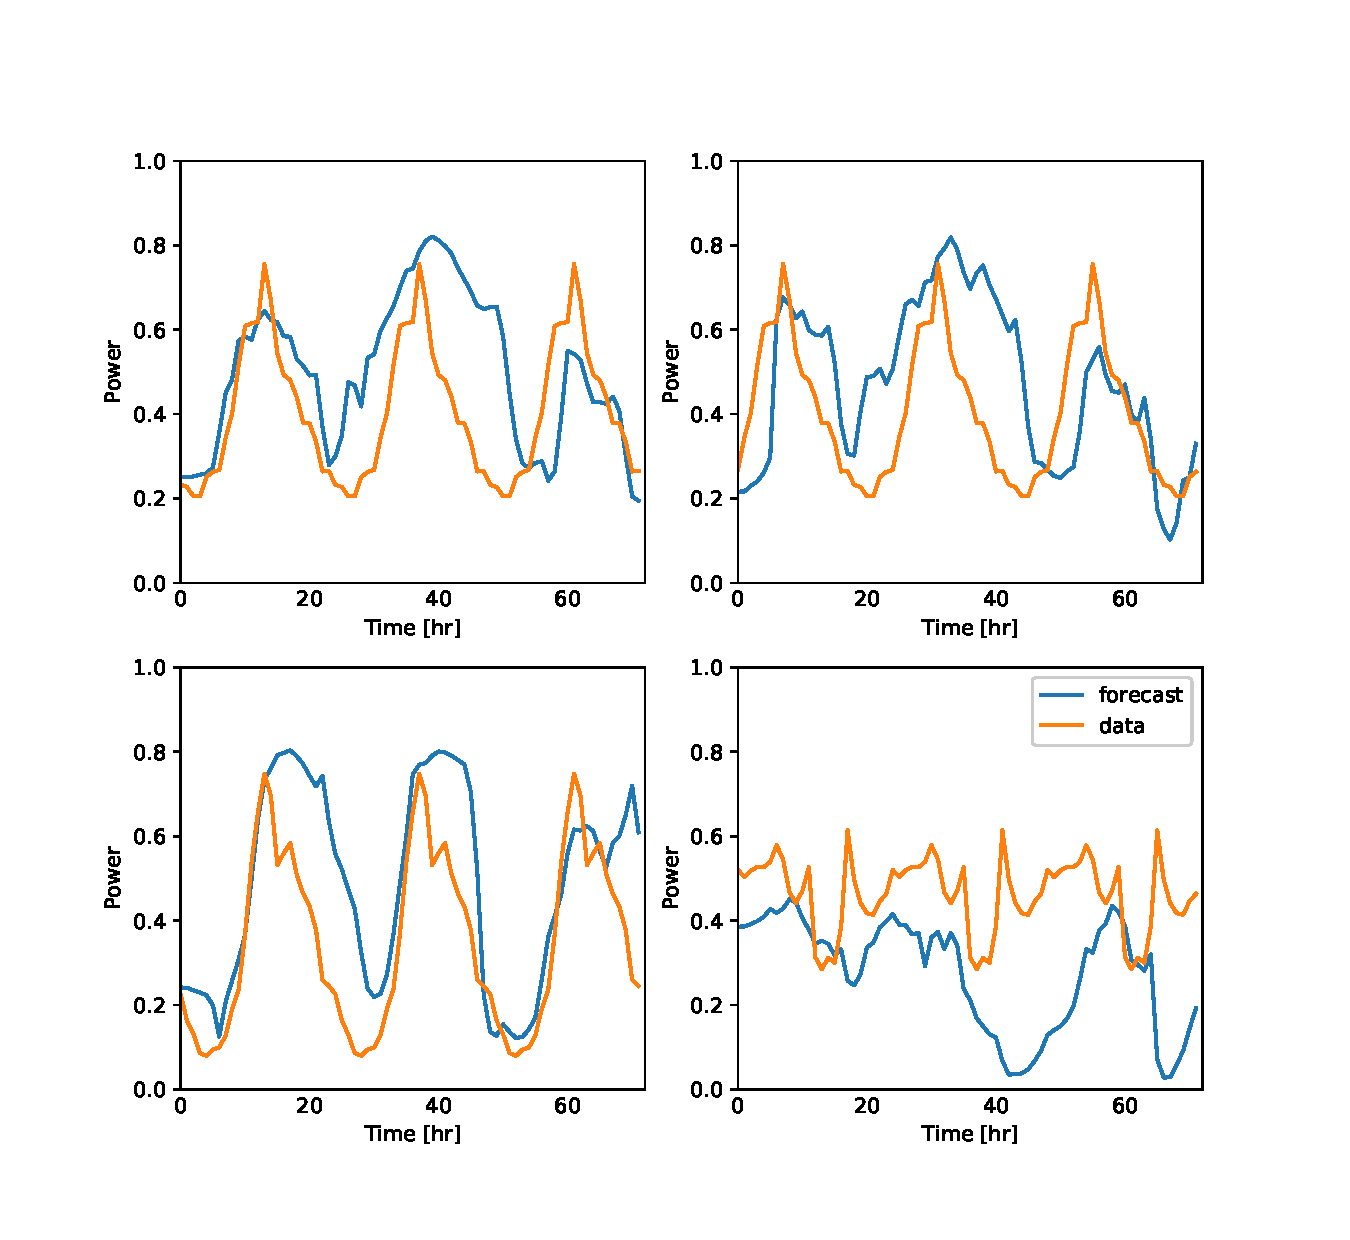
\includegraphics[scale=0.3]{Figures/forecast_data.eps}
  \caption{ Random selection of forecasts and their associated real power generation data }
  %\label{fig:boat1}
\end{figure}
\end{frame}


\begin{frame}\frametitle{ Forecast cubic splines interpolation }

For better numerical integration of the ODEs in order to find the moments of the stochastic process $V_t$, we need to interpolate between the discrete values of the forecast (as the given forecast is not fine-grained). \\


In this case, we choose to use cubic splines.

\end{frame}


\begin{frame}\frametitle{ Forecast cubic splines interpolation }

\begin{figure}
    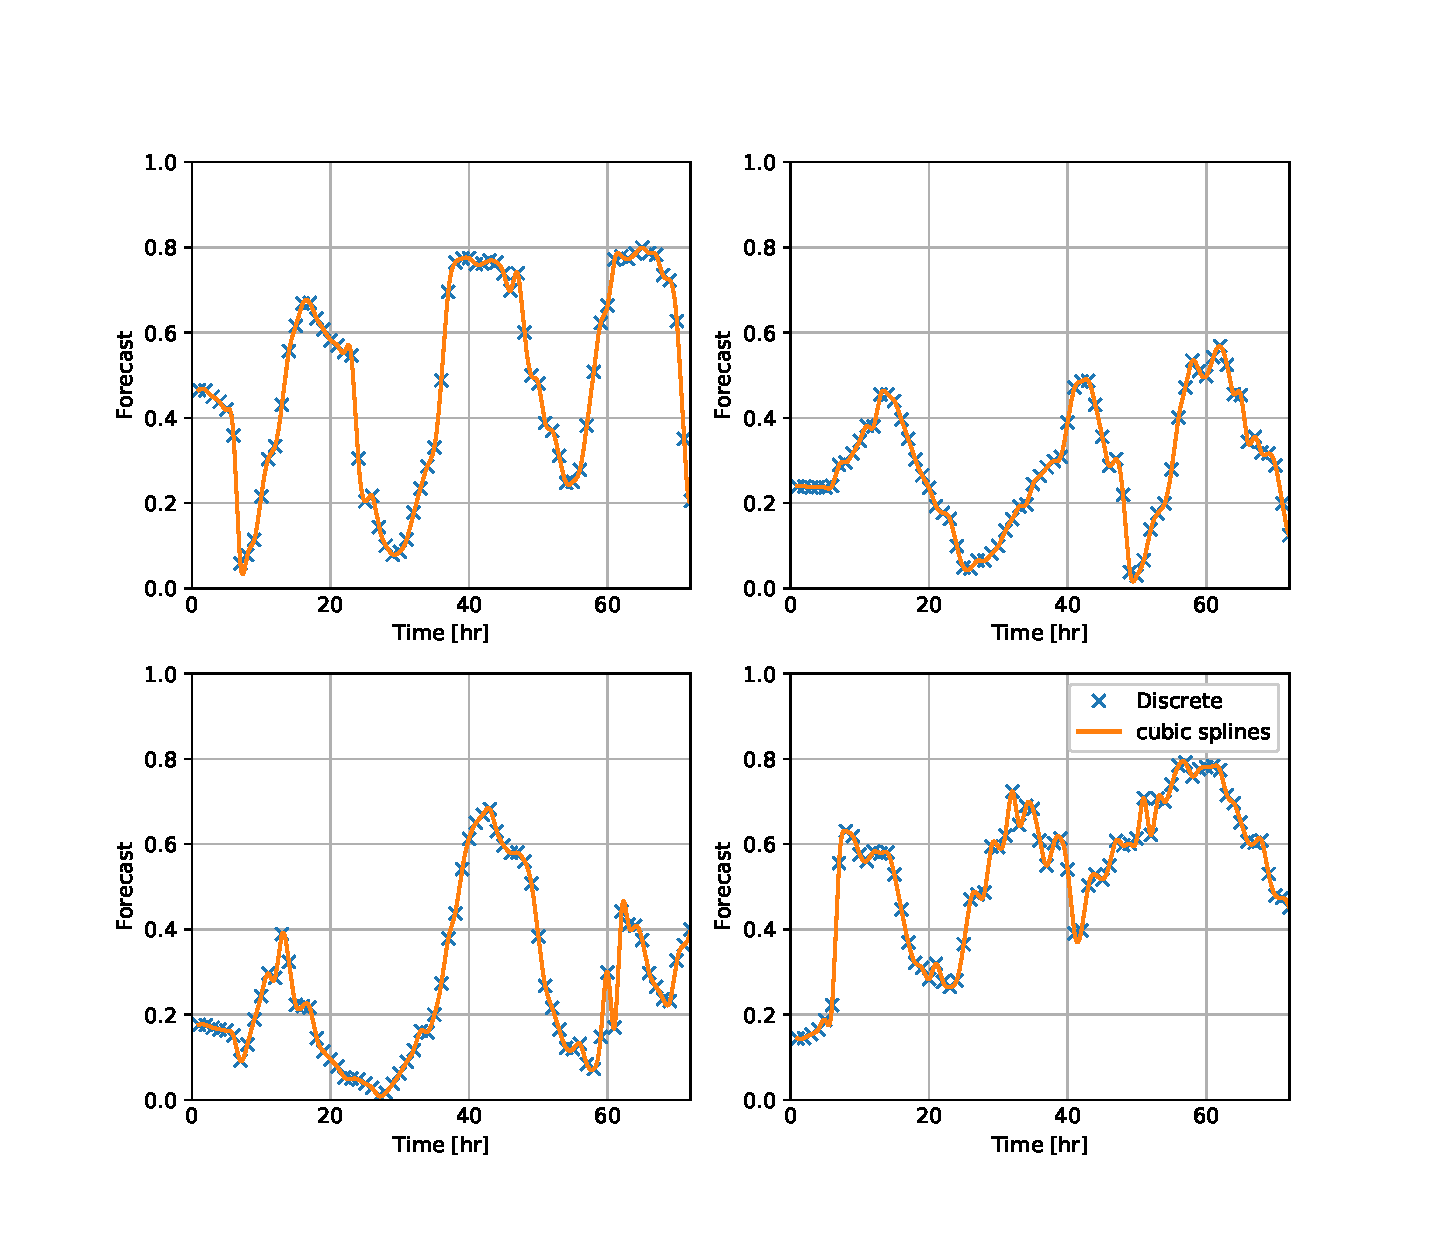
\includegraphics[scale=0.3]{Figures/forecast_splines.eps}
  \caption{  Random selection of forecasts discrete values and the associated cubic splines interpolation }
  %\label{fig:boat1}
\end{figure}

\end{frame}

%\begin{frame}\frametitle{ Case 4.1.1: Following a constant function - constant parameters }
%
%
%\end{frame}
%
%
%
%
%
%
%\begin{frame}\frametitle{ Case 4.2: Following deterministic functions - time dependent parameters }
%
%
%
%\end{frame}


\againframe{guide}



\end{document}






























